\documentclass[titlepage, 11pt]{article}
\usepackage{fullpage}
\usepackage[T1]{fontenc}
\usepackage[utf8]{inputenc}
\usepackage{lmodern}
\usepackage{graphicx}
\graphicspath{ {figures/} }
\usepackage{amsmath}
\usepackage[english]{babel}
\usepackage{csquotes}
\usepackage{enumerate}
\usepackage[margin = 2 cm]{geometry}
\usepackage{longtable}
\usepackage{setspace}
\usepackage{glossaries}
\usepackage{array}
\usepackage[titletoc,toc,title]{appendix}
\usepackage{biblatex}
\bibliography{11.bib}

\newcolumntype{L}[1]{>{\raggedright\let\newline\\\arraybackslash\hspace{0pt}}m{#1}}
\newcolumntype{C}[1]{>{\centering\let\newline\\\arraybackslash\hspace{0pt}}m{#1}}
\newcolumntype{R}[1]{>{\raggedleft\let\newline\\\arraybackslash\hspace{0pt}}m{#1}}
\makeatletter
\newcommand*{\rom}[1]{\expandafter\@slowromancap\romannumeral #1@}
\makeatother
%\renewcommand{\baselinestretch}{1.5}
\makeglossaries
\begin{document}
\begin{titlepage}

\newcommand{\HRule}{\rule{\linewidth}{0.5mm}} % Defines a new command for the horizontal lines, change thickness here

\center % Center everything on the page
 %	LOGO SECTION
%----------------------------------------------------------------------------------------
\begin{minipage}{0.4\textwidth}
\begin{flushleft} 

\includegraphics[width=50mm,scale=0.3]{ENAC.png}\\[1cm] % Include a department/university logo - this will require the graphicx package
\end{flushleft}
\end{minipage}
\begin{minipage}{0.4\textwidth}
\begin{flushright}
 
\includegraphics[width=60mm,scale=0.6]{TSE.png}\\[1cm]
 \end{flushright}
\end{minipage}\\[1.5cm]

%----------------------------------------------------------------------------------------
%----------------------------------------------------------------------------------------
%	HEADING SECTIONS
%----------------------------------------------------------------------------------------

\textsc{\LARGE ÉCOLE NATIONAL DE L'AVIATION CIVILE }\\[1cm] % Name of your university/college
\textsc{\LARGE TOULOUSE SCHOOL OF ECONOMICS }\\[1.5cm]
\textsc{\Large INTERSHIP REPORT}\\[1 cm] % Major heading such as course name
\textsc{\large Period: 02/05/2015 - 31/08/2015}\\[1.5cm] % Minor heading such as course title

%----------------------------------------------------------------------------------------
%	TITLE SECTION
%----------------------------------------------------------------------------------------

\HRule \\[0.4cm]
{ \huge \bfseries Innovation in Air Transport Market: Impact on Airlines' Competitive Behavior}\\[0.4cm] % Title of your document
\HRule \\[1.5cm]
 
%----------------------------------------------------------------------------------------
%	AUTHOR SECTION
%----------------------------------------------------------------------------------------

\begin{minipage}{0.4\textwidth}
\begin{flushleft} \large
\emph{Author:}\\
Aliya \textsc{Ussinova} % Your name
\end{flushleft}
\end{minipage}
~
\begin{minipage}{0.4\textwidth}
\begin{flushright} \large
\emph{Supervisors:} \\
Isabelle \textsc{Laplace} \\ % Supervisor's Name \\
Chantal \textsc{Latgé-Roucolle} % Supervisor's Name

\end{flushright}
\end{minipage}\\[2cm]

% If you don't want a supervisor, uncomment the two lines below and remove the section above
%\Large \emph{Author:}\\
%John \textsc{Smith}\\[3cm] % Your name

%----------------------------------------------------------------------------------------
%	DATE SECTION
%----------------------------------------------------------------------------------------

%{\large \today}\\[2cm] % Date, change the \today to a set date if you want to be precise

%----------------------------------------------------------------------------------------


\vfill % Fill the rest of the page with whitespace

\end{titlepage}
%\title{Internship Report}
%\author{Aliya Ussinova}
%\maketitle
\newcommand\tab[1][1cm]{\hspace*{#1}} 
\tableofcontents 
\listoffigures
\listoftables

\newpage 
\section{Basic professional context}\label{profcontext}
\subsection{Hosting organization: Ecole Nationale de l'Aviation Civile (ENAC)}
\doublespacing 
\tab Ecole Nationale de l'Aviation Civile (ENAC) is a public institution under the supervision of the French Ministry of Transport. ENAC provides education and professional training to prepare specialists in the domain of civil aviation. Starting from 1949, ENAC offers favorable environment for educational and research purposes in the field of air traffic management and aviation. Specialists from different fields: pilots, controllers, mechanics and researchers are located in the same campus and work together for development and promotion of technical and academic expertise. ENAC is one of the biggest grandes écoles d'ingenieur in aviation in the world, with 2000 student enrolled annually in full-time programs and 7500 interns following continuous training \cite{ENAC}.\\ 
\tab Research activities at ENAC are organized in 4 laboratories: MAIAA (Applied mathematics, computing and automatic for  aviation), TELECOM (Network, antennas and electromagnetism, GNSS), LII (Laboratory of interactive computing) and LEEA (Laboratory of economics and econometrics of aviation), as well as transverse research programs: Drones, Sustainable Development of Air Transport, Management of Air Control as well as General Aviation, Helicopters, Air Operation (AGHOPA). In parallel with research, there are 4 educational departments: Sciences and Engineering for Air Navigation (SINA), Languages and Social Sciences (LH), Air Transport (TA) and AIR Traffic Management (ATM) \cite{ENAC}.

\subsection{Project NECTAR}\label{NECTAR}
\tab NECTAR is one of the projects of synergy and exchange within the expertise of ENAC researchers. It is a joint product of laboratories MAIAA and LEEA, the research program - Sustainable Development of Air Transport, as well as the ENAC departments - SINA and TA. Air transport market is characterized by complex interactions between airlines, passengers, service providers, official regulators as well as countries. Moreover, the current global appeal for sustainable development poses challenges on airline industry to adapt their strategies in order to achieve operational efficiency and preserve high profits under the vigorous competition. NECTAR's objective is to contribute and deepen theoretical understanding of air stakeholders' behavior given the introduction of technological innovation, which allows to accommodate growing air traffic with lower impact on environment. One of the tasks made by ENAC in NECTAR is to assess the competitive reaction of airline companies to the introduction of the biggest passenger double-deck aircraft A-380. NECTAR project reunites joint effort of industrial giant - Airbus, the international research center - ONERA and école d'ingenieur l'ENAC.\\  
\tab The challenges, such as increasing air traffic and environmental issues, induce aircraft manufacturer, Airbus, to consider innovative solutions for the future generation of aircraft types. Their solutions will impact not only airlines companies, but the other participants of the air transport system. \\
\tab Even though this study takes the perspective of the aircraft manufacturer, the positive spillovers of it allows to enhance the ability to conduct multidisciplinary modeling of more complex situations, taking into account the diverse nature of the airline market participants. 
\section{Context and Objective of Internship}
\subsection{Current state of NECTAR Project} \label{Current Nectar}
\tab NECTAR has been launched in 2015. Previous to my arrival, my tutors - Isabelle Laplace and Chantal Latgé-Roucolle with the TSE intern - Ion Buzdugan, based on studies of \citeauthor{Givoni1} \cite{Givoni1} \cite{Givoni2}, \citeauthor{Pitfield} \cite{Pitfield}, have developed a conditional fixed effect logit model to evaluate the probability for an airline to use A-380 depending on the competitors use on the route Frankfurt-John F. Kennedy \cite{key}. They found positive and statistically significant relation  between the use of A-380 by airline company and the probability to introduce it by its competitors on the route. Moreover, they found positive relationship between the fuel price and the probability to use A-380, which is consistent with the results of previous studies that emphasized better fuel efficiency of larger aircraft.  
\subsection{Objective of the internship} \label{Objective Internship}
\tab There are several global goals that NECTAR aims to pursue. The first main question to which we are seeking the response is: given the introduction of the A-380 on airport market pair, do other companies have incentives to follow this innovation? The other question is whether after the introduction of A-380 there is a decrease in flight frequency due to higher capacity of airplane, allowing for better operational efficiency and lower level of carbon footprint. \\
%Even though there is significant number of studies covering the airline market, many of the papers do not evaluate the competitive aspect.
\tab Thus, in order to introduce new ideas into the model, the first objective of the internship is to perform a review of existing studies that covers the topic of our interest. The complete short summary of literature review could be found in table \ref{litreview} in Appendix \ref{Appendix}. \\
\tab The second objective of the project is to construct a database for the routes, where the A-380 is operated, in order to evaluate the robustness of the previously developed conditional fixed effect logit model. The main source of information is Official Airline Guide\cite{OAG}, the data and social factors are collected from other public sources such as World Bank. More details are provided in the section \ref{data composition} "Data composition" and Appendix \ref{Appendix}. \\
\tab The last objective of the internship is to define the econometric model(s) or to elaborate the existing one by testing new factors that might impact the probability to use the A-380. We base our analysis on the literature review that could explain and formulate the main characteristics of airline rationale given competition and innovation. 


\section{Inputs and valuable insights}\label{inputs}
\subsection{Literature Review} \label{literature review}
\tab My first contribution to the project was the accomplishment of literature review and collection of methodologies that could be further applied in this research. In 2013 the air transport activities contributed 12\% to transport and 2\% to total world $CO_2$ emission \cite{Emer1}. With rising global environmental concern and volatile oil prices, aircraft manufacturers aim to bring innovative technologies and adjust operation efficiency  of new generation of aircraft models. A-380 is one of such vivid examples. It is the biggest passenger aircraft that due to economies of size provides efficiency in terms of fuel burn, taking into account the classic seat configuration provided by the manufacturer \cite{King}. \citeauthor{King} (2007) \cite{King} in his analysis of A-380 highlights that the aircraft suits long-haul and high-density markets, allowing to absorb high-frequency operations. The author notes that if flying intelligently the aircraft can sustain markets in the periods of high fuel price by reducing the fuel cost per passenger kilometer. The reduction of frequency is directly linked to the reduction of fuel burn and correspondingly lower level of carbon emission. The increase in the size on the other hand does not provide intuitive answer whether emission per passenger decreases, which is the main intention and result that NECTAR project pursues. 
\\  The selection of scientific literature targeted the mentioned earlier objectives of NECTAR project: 
\begin{itemize}
\item Given operation of new aircraft A-380 by one of the airlines on the market, do other competitors have incentive to follow the innovation?   
\item If the air carriers introduce A-380 in their fleet does it lead to the reduction of frequency of flights? 
\end{itemize}
\tab Extending the above questions, there are different theoretical and empirical perspectives and focuses that have to be taken into account. The first question on competition implies the following theoretical concepts and frameworks:  
\begin{enumerate}
\item Strategic theoretical approach to innovation and competition
\begin{enumerate}[a)]
\item What does classical industrial organization theory can suggest about the incentives to follow innovation in airline market? 
\item How do we measure and classify competition among the airline companies? 
\end{enumerate}
\end{enumerate}
\tab During Master 1 in Industrial Organization course we have studied the link between innovation and market structure \cite{IO}, which became a useful takeoff point in my internship. In our case the innovation is not performed by the company itself, it is a technology acquiring innovation, where the firm not active on the market (Airbus) develops a technology and then firms decide whether to acquire it or not. The willingness to pay and acquisition of the technology depends whether the firm can further improve on its profit. In classical industrial theory there are two incentives for innovation:  
\begin{itemize}
\item[--] Profit incentive called by Jean Tirole pure incentive to innovate \cite{IO}	
\item[--] Strategic incentives such as competition between big firms or potential competition between entrant and incumbent \cite{IO}
\end{itemize} 
\tab Considering the main research questions in strategic context, I found useful the article of \citeauthor{aghion} \cite{aghion}, that formulates theoretical model in terms of present value of future profits. He defines level of profit when the competitors have the highest incentive to catch up and escape the competition. His main conclusion is that neck-and-neck industries are more prompt to introduce or follow the innovation for any level of competition. Even though the empirical implementation of this paper is not possible in our case due to the absence of detailed and precise information on profits for companies, this paper allowed to deduce hypothesis that probability to follow  innovation (aircraft A-380) will be higher for routes with neck-and-neck competition\footnote{Each route (airport origin-destination pair) is considered to be as a separate market}.\\
\tab Moreover, the behavior of firms is shaped by the competitive features that characterize market. The most popular approach to measure level of competition is the Herfindahl-Hirschman Index (HHI), calculated by adding the squared market shares \cite{Investopedia}:
\begin{equation}
HHI = s_1^2+s_2^2+...+s_n^2\footnote{Where $s_i$ is the market share of firm $i$ on the market}
\end{equation}
The values close to 1 indicate perfect monopoly, the values close to 0 - perfect competition. Researchers in their studies use number of competitors on the route or number of destinations to which airline flies as the proxies for competition. In this project these indicators will be tested and analyzed in order to identify the most sensitive index that is able to capture the competitive nature of airline companies. \\ 
\tab 
\begin{enumerate}
\setcounter{enumi}{1}
\item The empirical examples of green innovations in airline industry
\end{enumerate}
\tab The other important aspect is to study the how the scholars address the behavior of aviation sector under environmental constraints.The studies reviewed studied one of the following general ideas:
\begin{enumerate}[a)]
\item The influence of aircraft type and size on fuel consumption and $CO_2$ emission 
\item Current fuel and operational efficiency of airline companies
\item Airline fuel efficiency  given the environmental tax (carbon fee)\footnote{Carbon fee is the amount that is taxed depending on the level of $CO_2$ emitted by the company during operation}
\end{enumerate}
\tab While studying the fuel emission some authors take a company-specific approach or industry as a whole and others consider the effect on passenger demand. \citeauthor{Emer1} \cite{Emer1} identify that pressure from competitors and strict governmental regulations are the driving forces for innovation in airline industry. They study how environmental innovations affect the companies financial and operational performance. Based on their classification of innovation into technology and process based, we could classify introduction of A-380 as a process-based innovation, which allows to improve operational efficiency by decreasing cost per transported passenger. The other scholars (\citeauthor{COEurope} \cite{COEurope}, \citeauthor{seatconfig} \cite{seatconfig}, \citeauthor{larger} \cite{larger}, \citeauthor{threeMarket} \cite{threeMarket}) focused on the relationship between aircraft size and environmental productivity, arriving to the conclusion that larger aircraft provides improvement in efficiency and that there is an overall trend in change to larger aircraft types for short and medium haul flights. These articles were useful since they provided valid conclusions on the efficiency of larger aircraft. \citeauthor{carbon} \cite{carbon} use interesting independent variables, which will be tested in our case. These are hub\footnote{Dummy variable, indicating 1 if the airport is a connection hub and 0 otherwise}, airline\footnote{dummy variables for airlines, capturing the preference of consumers on specific airlines}, aircraft size, alternative airport\footnote{dummy indicates the presence of alternative airport in vicinity of the city}, fuel consumption\footnote{fuel consumption per passenger}. The authors also come up with creative instruments to tackle endogeneity for market share. These are market related instruments(number of airlines on the market, number of offered connections), route-level instrument (if the airport is hub for the operating airline) and rival related instruments (percentage of non-stop rival routes\cite{carbon})\\
\tab Another popular approach is to study the effect of the introduction of environmental tax or $CO_2$ emission cap\footnote{$CO_2$ emission cap is the maximum allowable amount of emission. Companies can purchase allowances and trade them if permitted level is not achieve} on the behavior of the airlines companies. \citeauthor{carbon} \cite{carbon}, introduce the model with hypothetical environmental tax and analyze how it will affect the demand side of air traffic given the different price elasticies of demand. The other types of studies (\citeauthor{ETSItaly} \cite{ETSItaly} \citeauthor{demandBusiness} \cite{demandBusiness}, \citeauthor{ETS22} \cite{ETS22}) focus on change of airline efficiency after the inclusion of aviation industry into European Union Emission Trading Scheme, the first largest greenhouse gas emission controlling organism \cite{ETSEU}. ETS pushes European airlines companies to reduce pollution in order to sustain emission at stable level given the increase in passenger traffic. Initially these papers encouraged us to incorporate the policy of external regulator in the model. However, in most cases A-380 operates long-haul international flights, whereas ETS does not apply to non-EU airline companies. At the outset of ETS the EU aimed to impose tax on any airline landing within the EU, however, due to external international pressures, EU postponed its universal application and currently raises taxes only from EU airlines. Thus, in our case implementation of tax and representation of its effect on airline behavior is not feasible. \\ 
\tab 
\begin{enumerate}
\setcounter{enumi}{2}
\item Market share and frequency share modeling for airline market
\end{enumerate}
  \tab The second NECTAR's objective that we aim to achieve, requires the framework for modeling the competitive interaction between airline companies. \citeauthor{marketshare} \cite{marketshare} notes that airline companies by increasing market share have higher probability of profit maximization and there are two strategies that airlines can follow, which are either to increase frequency or to increase seating capacity with larger airplanes. They also note that efficiency is a likewise important factor that impact market share. The paper outlined the variables that affect market share. These are the average price tickets, alliances membership, number of competitors per destination, load factor, that also will be tested in our model. \citeauthor{Pai} \cite{Pai}, \citeauthor{Wang} \cite{Wang} and \citeauthor{Bilot} \cite{Bilot} examine the frequency strategies and aircraft sizes. \citeauthor{Wang} \cite{Wang} found that in emerging markets airlines adjust the growing traffic by increasing frequency. They also concluded that more concentrated\footnote{More concentrated refers to the concentration in terms of HHI (HHI close to 1), when there are less number of carriers} market structures resulted from merges lead to the reduction of frequencies. Therefore, the alliance membership will be also incorporated in the our model. \\
\tab Even though scholars approached the topic from different angles, the collected findings demonstrate that international environmental concern did not bypass aviation industry. Airline companies had to adopt efficient strategies to sustain their competitiveness under the conditions of volatile and dynamic market.  

\subsection{Database} \label{Database}
\tab The database used during the internship is the OAG schedule analyzer - database of Official Airline Guide, which is a UK company that provides airline data services \cite{OAG}. It is a powerful tool, which contains the past, current and future information on supplied scheduled flights. Being first published in 1929, today OAG holds information for 1000 airlines and 4000 airports. The advantage of Schedule analyzer is that it allows to view  activities of competitors on different routes and obtain information on the relative share of supply. It contains different variables such as airports, carriers, flight frequencies, aircraft types, alliance etc. This is one of the most comprehensive and widely used data on traffic flow. The disadvantage of this database is that it contains only scheduled flights. The unscheduled flights do not enter into database and the observations for canceled flights are not deleted. Therefore, when combining the OAG data (supply) with data on the demand (annual traffic flow from origin to destination), it is not possible to get the accurate estimation for load factor.\\ 
\tab The ENAC database on Air Transport is also useful for our analysis. The ENAC database contains information for 500 airline companies and consist of three separate databases on Airlines companies, Airports and Traffic flows. It contains data on different indicators from various sources (\citeauthor{IATA} \cite{IATA}, \citeauthor{ICAO} \cite{ICAO}, Airline \citeauthor{AirlineMonitor} \cite{AirlineMonitor}, etc), thus, providing an opportunity to compare the validity of data. ENAC database was used to extract data on the demand-side, namely the actual recorded traffic flow and financial indicators of companies performance (annual revenues and profits).  \\ 
\tab The last data set is related to the fuel consumption. It was generated using simulation software created by Cyril Allignol, an ENAC researcher, based on Base of Aircraft Data (BADA) and EUROCONTROL methodology \cite{BADA}. The software calculates the fuel consumption based on type of aircraft, distance flown, flight altitude and total take-off weight. It provides good approximation with real values. The example of the estimation and illustration of the software is provided in Appendix \ref{Appendix} section \ref{BADA appendix}.  

\subsection{Database Composition} \label{data composition}
\tab In our example, the type of data is panel data. Besides having cross sectional and time series dimension, our panel data has more complex hierarchical form \cite{Hsiao}: the dependent variables y measures the frequency of flights or the probability to follow the innovation for the airline $i$ on Origin-Destination route $j$ at time $t$.  The panel structure was chosen due to the following advantages\cite{Hsiao}: 
\begin{itemize}
\item[--] It allows to conduct more precise inference due to higher variability: presence of greater number of observations allows for more degrees of freedom \cite{Hsiao}.
\end{itemize}
\tab Moreover, by capturing inter- and intra- individual characteristics with panel data, it is possible to model more complex behavior. In our case it is an important aspect, since the change of aircraft is not an immediate process, it takes several months or years for companies to adopt new fleet. Thus, the timing allows to capture the response dynamics to follow innovation. Moreover, since we have an ordered observations, after the fleet change the company $i$ will continue its operation in future, therefore, time series component of the data exhibits high correlation with lagged values.
\begin{itemize}
\item[--] Panel data allows to control the omitted variables \cite{Hsiao}
\end{itemize}
\tab By capturing effect between individuals and their behavior over time we are able to legitimately ignore the impact of omitted variables that are constant over time. These could be company or route-specific characteristics that are not observable in our case. 
Time-series dimension of panel data captures the dynamics of development, since market entrance merge and exit are common practices in airline industry. Thus, we are able to control highly dynamic and rapidly changing competition structure of the market.\\
\tab However, along with all the benefits of panel structure, there are potential issues that could lead to biased estimation of coefficients of regression model. Often time-series data exhibits seasonal behavior \cite{Hsiao}, which is the case for airline market. Depending on the route, there are particular periods when passenger traffic increases substantially due to vacation, business seasons etc. The graph \ref{season} shows that seasonality is a common feature for the routes in our sample: 

\begin{figure}[ht]
\centering
\caption{Seasonality on some routes}
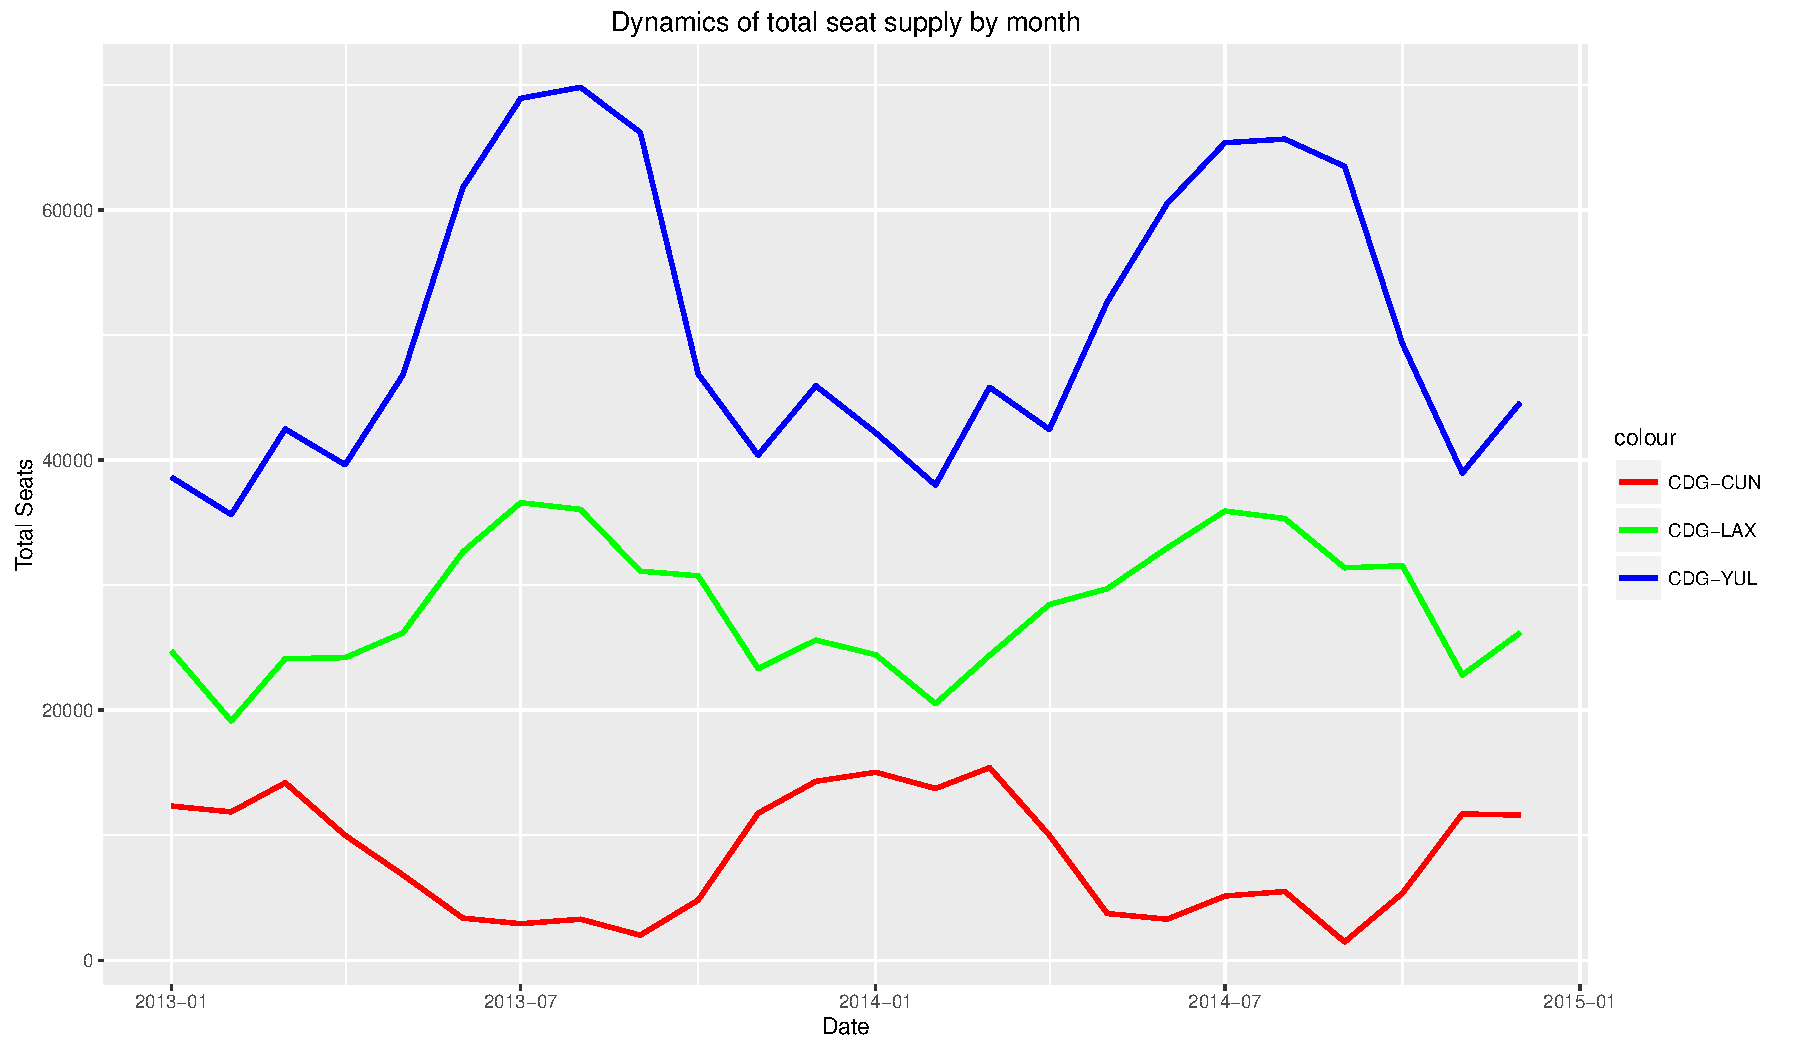
\includegraphics[width=200 mm]{Rplot07.pdf}
\label{season}
\end{figure}
\tab As it could be seen from the figure \ref{season} there is a clear seasonal trend in all of three routes, however, the pattern is not the same\footnote{Blue line corresponds to the airport pair of Paris-Montréal, green - Paris-Los Angeles, red - Paris-Cancun.}. For CDG-LAX, CDG-YUL routes we see that seats surge dramatically for summer periods with peaks in July-August, whereas for CDG-CUN the highest points comes in December-January. This is not a surprising fact, people travel to Los Angeles and Montréal in summer period, whereas Mexico is the more favorable for tourism during winter. \\
\tab Seasonality will be corrected in this study either by sub-setting observations for particular period (for example one month or quarter), or by regressing the variables that exhibit seasonality on a set of seasonal dummies \cite{Hsiao}. 
\\
\tab The other potential problem is the trending of independent variables. Overall, there is an annual increase in passenger traffic, as shown in figure \ref{traffic}: 
\begin{figure}[h!]
\centering
\caption{Growth of passenger flow}
\label{traffic}
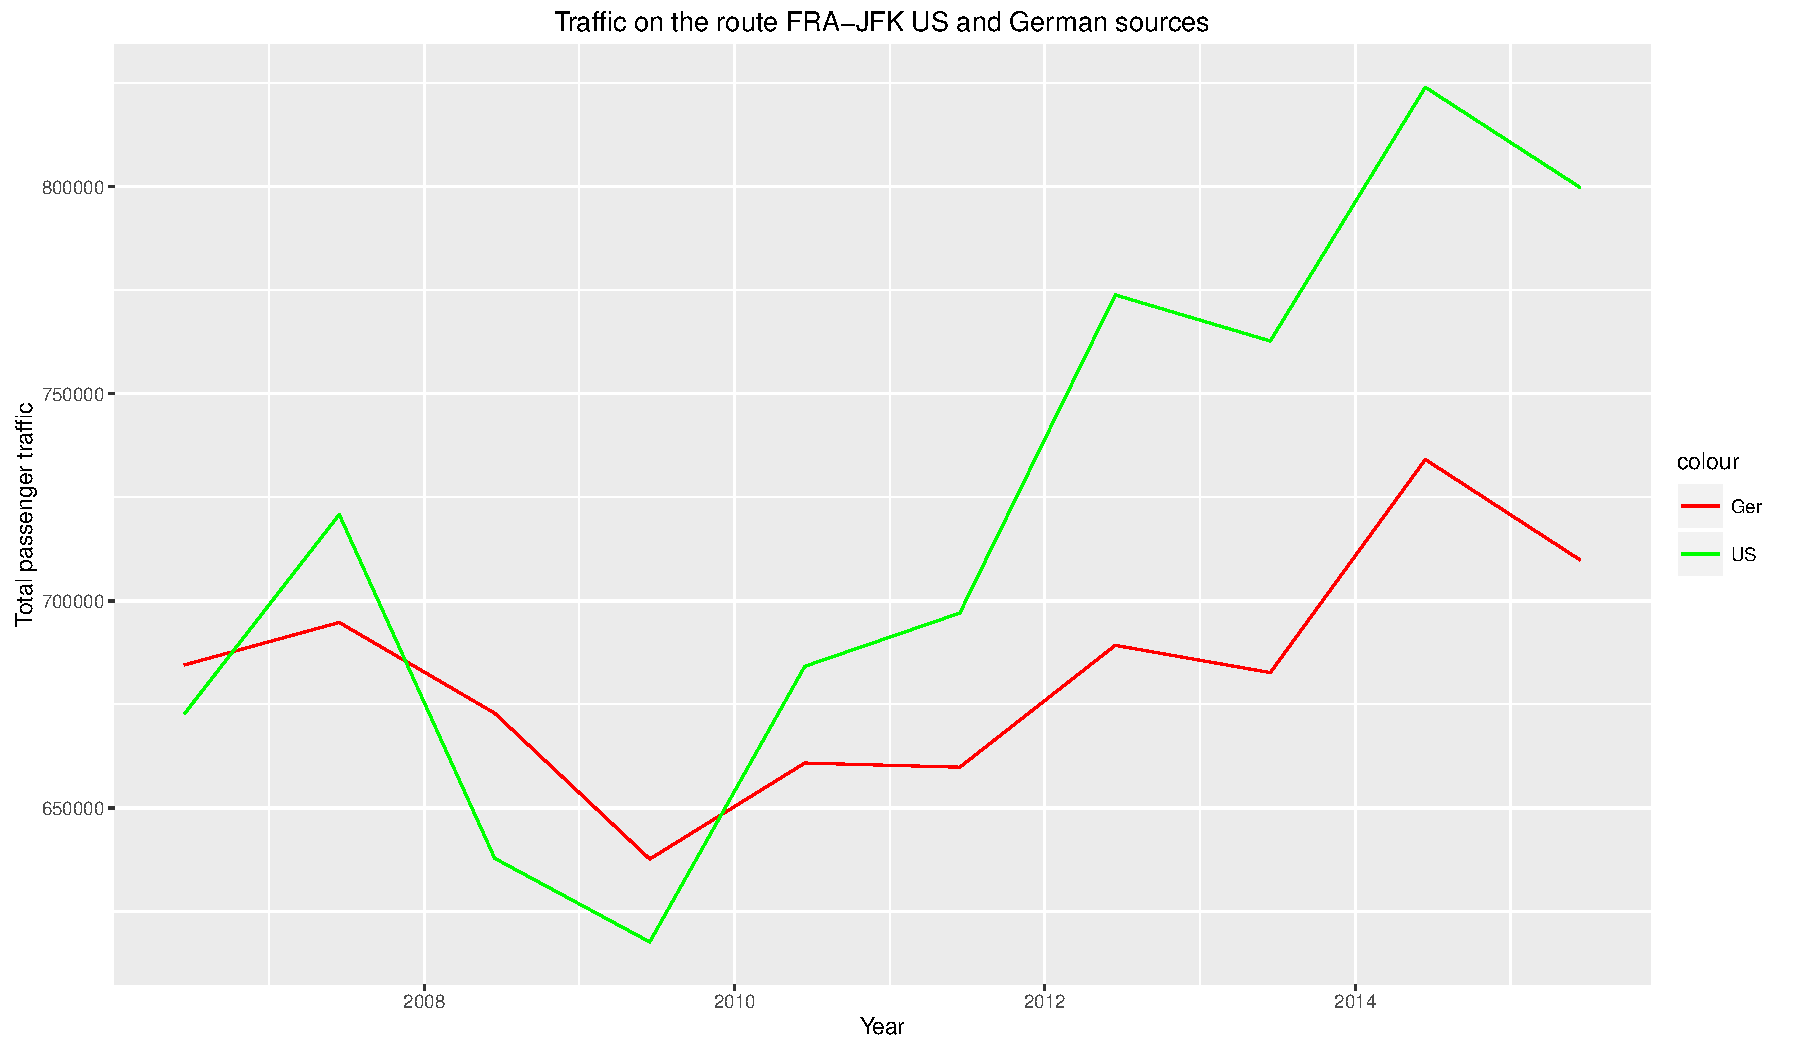
\includegraphics[width=200 mm]{traffic1.pdf}
\end{figure}
\\
\tab Despite the shock in 2007 to 2009 on figure \ref{traffic} due to global financial crisis, there is an upward trend, which is consistent with predictions of scholars that in future passenger flow will continue to increase. Therefore, in our model we will control for special events and shocks using dummy variables for particular period when a shock occurred.\\
\tab One should suspect trend if the $R^2$ is very high. If the trend is detected visually or analytically, one way to correct for it is by adding linear trend \cite{Hsiao}:
\begin{equation}
y_{it} = \beta_0+ \beta_1x_{it1} + \beta_2x_{it2} + ... +\beta k_it + u_it
\end{equation}
\tab Omitting the trend could lead to biased estimates, specially if the other regressors are also trending. Thus, keeping in mind these potential issues with our data, during the next weeks of internship, the goal is to produce valid, robust model with unbiased estimators.   \\
\tab In total there are 151 airport-to-airport routes on which A-380 aircraft operates. After splitting the data on monthly bases for the last 10 years, there are 44767 observations. The descriptive statistics of the up-to-date data set is presented in table \ref{descriptstat}:
\begin{table}[!htbp] \centering 
    \caption{Descriptive statistics of data set} 
  \label{} 
\begin{tabular}{@{\extracolsep{5pt}}lccccc} 
\\[-1.8ex]\hline 
\hline \\[-1.8ex] 
Statistic & \multicolumn{1}{c}{Mean} & \multicolumn{1}{c}{St. Dev.} & \multicolumn{1}{c}{Min} & \multicolumn{1}{c}{Max} \\ 
\hline \\[-1.8ex] 
distance\_km & 5,390.288 & 3,430.822 & 346 & 13,802 \\ 
frequency & 59.665 & 58.207 & 1 & 548 \\ 
frequency\_share & 38.218 & 29.087 & 0.130 & 100.020 \\ 
total\_seats & 16,425.410 & 14,236.030 & 124 & 128,663 \\ 
freight\_tonnes & 958.401 & 1,340.844 & 0.000 & 12,510.400 \\ 
seats\_A380 & 1,710.438 & 5,826.298 & 0 & 79,980 \\ 
freight\_tonnes\_A380 & 116.688 & 542.282 & 0.000 & 9,749.500 \\ 
HHI  & 0.462 & 0.241 & 0.134 & 1.000 \\ 
Monopoly & 0.113 & 0.317 & 0 & 1 \\ 
total\_tonnes & 1,738,381.000 & 1,509,170.000 & 12,400 & 13,293,790 \\ 
\hline \\[-1.8ex] 
\multicolumn{5}{p{.8\textwidth}}{\textit{Notes}: N=44767}
\end{tabular} 
\label{descriptstat}
\end{table} 

\tab The data set is still in the process of modification with more variables being added in the following weeks. As it could be seen from the above table \ref{descriptstat}, A-380 serves long-haul routes with average distance of the route - 5390 km. The average frequency per airline serving the route is 59 flights per month. On average the routes have oligopoly market structure (HHI=0.46), however, there are routes that are entirely supplied by single carrier\footnote{Monopoly variable is a dummy variable equal to 1 if there is one carrier on the route and 0 otherwise} . 


\section{Conclusion}\label{conclusion}
\tab This report presents the overview of activities performed during the first month of the internship. The report outlines the main results and conclusions contributed to NECTAR project, which investigates the competitive response of airline companies on the introduction of A-380. The further extension is to test the econometric models on sample of routes (151 routes) and to analyze the significance of other variables found in literature review. The model is a starting point in the analysis of behavior of airline companies and environmental benefits that operation of A-380 generates. The goal for the next month is to identify whether the larger size of aircraft A-380 leads to the reduction in frequency of flights and reduces the $CO_2$ emission per seat, as well as to study to what extend A-380 can contribute to the evolution of more sustainable air transportation system. 
 
\singlespacing
\newpage
\begin{appendices}
\section{}\label{Appendix}
\subsection{Information about A-380} \label{A380info}
\tab A-380 is the biggest passenger aircraft. By introducing this model Airbus aims to meet the future demand for "more-efficient, cleaner, quieter and smarter" aircraft \cite{Airbus}.  % Add a reference 
With typical 4-class configuration A-380 provides seats for 544 passengers, with possible maximum of 853 people transported at once. 

\subsection{Information about OAG} \label{OAGinfo}
\tab The OAG Schedule analyzer provides the most recent data on the scheduled flights \cite{OAG}. OAG report allows to analyze the routes on which airlines operate aircraft A-380 based on dimensions and metrics responding to the need of the search. Below is the example of data extraction based on the selected criteria. We included into database observations of operating carriers on routes where A-380 was used \footnote{In this example airport-market-pair Frankfurt-John F. Kennedy is illustrated}. We included only one-way observations, since two-way is a multiple of one-way schedule. The observations are collected on monthly basis from January 2005 to December 2015
\begin{figure}[h]
\centering
\caption{OAG interface}
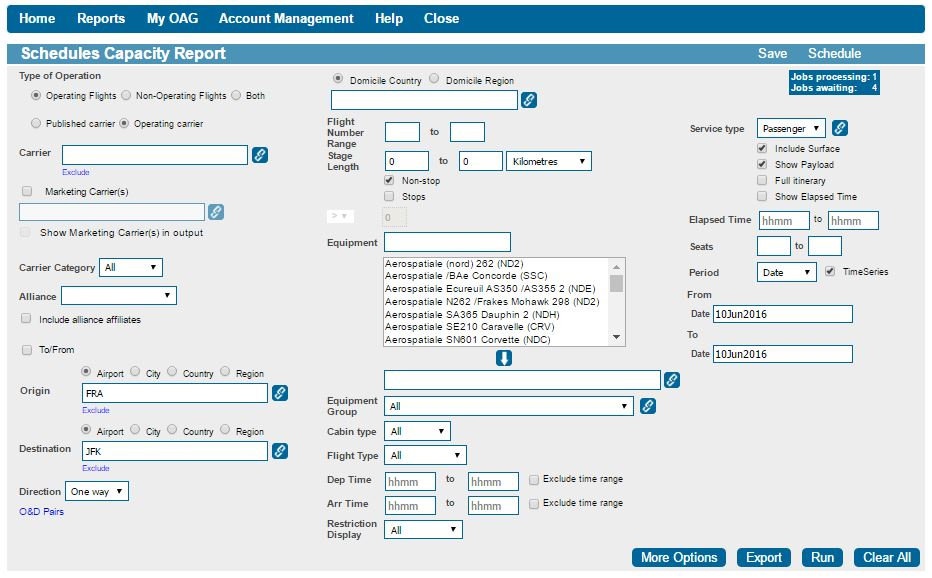
\includegraphics[width=150mm, scale = 1]{OAG.JPG}
\end{figure}
\subsection{BADA: Jet fuel consumption simulation}\label{BADA appendix}
An image below is the example of the simulation with BADA software \cite{BADA}. The first input is the model of aircraft (A-388), the second is the distance flown (6186), the third is the altitude of cruise phase and the last is the total take-off weight, which corresponds to maximum takeoff weight. In the output the data for flight time and fuel consumption is calculated. 
\begin{figure}[h!]
\centering
\caption{BADA software interface}
 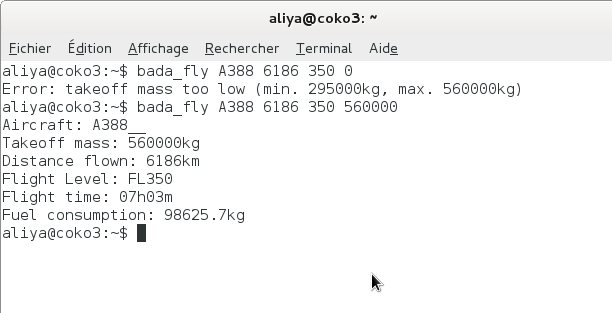
\includegraphics[width=150mm,scale=1]{Cap2.png}\\
\end{figure}
\newpage
\subsection{Literature review summary}

\begin{footnotesize}
\begin{longtable}[h]{|  C{1 cm}  C{1cm}  C{1cm}   C{2cm} C{4cm}  C{5cm}|}
\caption[]{Literature review \label{litreview}}\\
\hline
\textbf{Papers} & \textbf{Airlines} & \textbf{Period} & \textbf{Methodology} & \textbf{Outcome} & \textbf{Why it is useful for us} \\[15mm]  \hline
Wei \cite{Emer1} & 40 airlines from Emerging countries & 2012 & OLS and Logit. Financial performance regressed on innovations and other variables & Technology-based and process- based innovations increase revenues, only process-based increase profit, because the former is costly. Process-based innovations positively affect load factor of airlines. & Ideas for independent variables such as innovation measured as a ratio of aircraft that have this innovation. Control variables that could be tested in our paper are fleet age, airline size, competition expressed as number of destinations to which airline flies. Since larger aircraft is a process-based innovation, we can use conclusions from this paper. \\[15mm] 
Scotti \cite{COEurope} & 18 European airlines & 2000-2010 & OLS model. Efficiency as Biennial Malmquist Luenberger -(BML) index regressed on network characteristics and fuel efficiency & Airlines can boost productivity by introducing bigger aircraft. Increase in load factor increases productivity. Greener aircraft is the primary way to increase environmental productivity & Useful approach to measure environmental productivity. The ideas to test in our model variables that they have used. They came up with the conclusion that larger aircraft help to decrease $CO_2$ emissions \\[15mm] \hline
Hsu and Wen \cite{Fuzzy} & China airlines & 2000 & Fuzzy logic based & Higher load factors leads to airlines determining lower flight frequencies of larger aircraft & Programming approach to model flight frequencies under the competitive equilibrium \\[15mm] 
Devriendt \cite{load} & Airlines in OAG data & Jan - Aug 2001 & Merging demand and supply data to calculate the load factors & The database clearly underestimates load factors. There are potential issues with data sets such as absence of information on non-scheduled flights etc. & They come up with creative approaches to aggregate data. Their approach will be used to manipulate our data and calculate load factors in the routes of our interests \\[15mm] 
Pagovi et al \cite{carbon}& US airlines & first quarter of 2012 & Nested logit model. Game-theoretic approach & After implementation of carbon policy the airlines increase ticket prices leading to demand fall from 2.4 to 21\% depending on carbon fee & They provide good modeling of the airline market (demand and supply) and come up with creative ideas to tackle endogeneity \\[15mm]
Park et al \cite{seatconfig} & Over the world & 2012-2013 & Calculation of fuel burn as a function of aircraft type for a particular route & Fuel efficiency depends on stage length and seat configuration but the larger is the plane the more fuel use decreases & We will use their approach to estimate fuel consumption based on aircraft type and route \\[15mm] 
Zou et al \cite{US} & 15 US jet airlines & 2010 & Ratio-based, deterministic and stochastic frontier approaches & Fuel efficiency improvement can provide cost savings up to 2 and 3 billion US dollars based on different approaches. & They make useful conclusions that we can use for literature review but not the model itself \\[15mm] 
Babic et al \cite{marketshare} & Eastern European Airlines & 2001-2012 & OLS to determine the variables that affect market share and Fuzzy logic to model market share & The two significant variables that affect market share are frequency share and number of competitors per destination at the airport. After training on the data they achieved estimated results close to real & It is useful since it identifies explanatory variables that affect the market share the most \\[15mm] 
Morell \cite{larger} & 7 US airlines &  & Log-Log regression models with dependent variable fuel per seat and independent variable total seats or kg & There is a strong relationship between fuel efficiency and size & This paper is useful since it considers fuel efficiency and aircraft size, we can conduct similar testing with A-380 and compare with other aircraft types \\[15mm] \hline
Miyoshi and Mason \cite{threeMarket} & EU-UK, US-EU& 2004 & Estimation of $CO_2$ using two-stage approach: landing-takeoff and cruise stages & The difference between ratio of covered demand transported by airline and total emission depends on aircraft used, stage length, load factors and cabin configuration & Most of the analysis is done in form of graphs and we can consider their approach for estimation of $CO_2$ emission. \\[15mm] 
Amizadeh et al \cite{commerSixlargest} & 6 EU airlines & 2010-2013 & $CO_2$ emission with respect to different business models & The most $CO_2$ efficient business models are Charters, LCC, Regionals. Despite the increase in traffic the efficiency improves from 1\% to 4.5\% & This paper gave idea to integrate the evolution of traffic flow into the model \\[15mm] 
Li et al \cite{ETSItaly}& 22 airlines & 2008-2012 & SMB and Dynamic DEA models & Efficiency of non-European airlines are much lower than for European ones. The inclusion of airlines into EU ETS forces to improve fuel efficiency to cope with limited carbon emission permits & They nice cope with absence of information and collected it from annual reports, which could be done in our case as well \\[15mm]
Meleo \cite{ETS22} & Italian airlines & 2012-2014 & Formulas for calculating total direct costs, profits and emission & Even if EU ETS carbon fees are 100\% passed onto passengers the final price will increase less than 1\% . Even thought Italian airlines revenues fell it was not due to EU ETS policies & They provide how to compare scenarios if there is an introduction of carbon tax on airlines based on level of emission. This approach could also interesting to consider for A 380 \\[15mm] 
Lu \cite{demandBusiness}& LHR-AMS and LHR-CDG routes &  & Formula for emission calculation, environmental charge and elasticies & Depending on the price elasticies of leisure and business markets the author found different values for  decrease in demand resulting from increase in price. The values range from 0.9 to 7.8\% reduction in demand & This paper gave idea to consider also price elasticies of demand and the type of business models such as network carrier low costers etc. \\[15mm] 
Grimme \cite{economicImpact} & Ryanair, Lufth., Cordon and Air Dolom. & 2008-2012 & Model for future carbon dioxide emission cost of acquiring allowance  and demand & Network carriers can pass more of environmental costs onto passengers than LCC, holiday carriers and regionals. Nonetheless, the financial success of LCC is not likely to be affected & This is a future predictive model, it could be used as a starting point if we will introduce environmental tax in our model \\[15mm] \hline
%\end{tabular}
\end{longtable}
\end{footnotesize}




\end{appendices}


\newpage
\printbibliography
\end{document}
